\documentclass[12pt]{article}
\usepackage[utf8]{inputenc}
\usepackage[english]{babel}
\usepackage{amsmath}
\usepackage{natbib}
\usepackage{graphicx}
\usepackage{hyperref}
\usepackage{caption}
\usepackage{caption,float}
\usepackage[vmargin=3cm,hmargin=3cm]{geometry}

\begin{document}

{\centering

\rule{\textwidth}{1.6pt}\vspace*{-\baselineskip}\vspace*{2pt} 
\rule{\textwidth}{0.4pt}\\[\baselineskip] 
{\LARGE Autorank - a simple python package}
\rule{\textwidth}{0.4pt}\vspace*{-\baselineskip}\vspace{3.2pt}
\rule{\textwidth}{1.6pt}\\[\baselineskip] 

\vspace{20mm} %5mm vertical space
\scshape % Small caps
CMSC 6950 - Computer Based Research Tools and Applications \\ [\baselineskip]
Term Project \\[\baselineskip] 
6th August, 2020 \\[\baselineskip] 
\vspace{20mm} %5mm vertical space
Submitted by \\[\baselineskip]
{\Large Anne Odeh \par}
\vfill
{\itshape Memorial University of Newfoundland \\ St. John's, Canada.\par} 
}

\newpage

{\centering
  \section*{Abstract}
}
Reproducibility is seen as one of the pillars of the entire scientific method, a criterion on which to measure the efficacy of an experiment. This paper presents how autorank can be reproduced by understanding how it works and the necessary tools that are required to mimic its exact work. \\\\


\section{ Introduction}
Autorank is a simple Python package with one task: simplify the comparison between (multiple) paired populations. This is, for example, required if the performance different machine learning algorithms or simulations should be compared on multiple data sets. The performance measures on each data set are then the paired samples, the difference in the central tendency (e.g., the mean or median) can be used to rank the different algorithms. This problem is not new and how such tests could be done was already described in 2006 in the well-known article Janez Demšar. 2006. Statistical Comparisons of Classifiers over Multiple Data Sets. J. Mach. Learn. Res. 7 (December 2006), 1–30.\\\\
Regardless, the correct use of Demšar guidelines is hard for non-experts in statistics. Correct use of the guidelines requires the decision of whether a paired t-test, a Wilcoxon's rank sum test, repeated measures ANOVA with Tukey's HSD as post-hoc test, or Friedman's tests and Nemenyi's post-hoc test to determine an answer to the question if there are differences. For this, the distribution of the populations must be analyzed with the Shapiro-Wilk test for normality and, depending on the normality with Levene's test or Bartlett's tests for homogeneity of the data. All this is already quite complex. This does not yet account for the adjustment of the significance level in case of repeated tests to achieve the desired family-wise significance. Additionally, not only the tests should be conducted, but good reporting of the results also include confidence intervals, effect sizes, and the decision of whether it is appropriate to report the mean value and standard deviation, or whether the median value and the median absolute deviation is more appropriate.


\newpage
\section{Reproducing autorank}
I was able to reproduce autorank by running the example code provided:
\begin{figure}[!htbp]
	\centering
	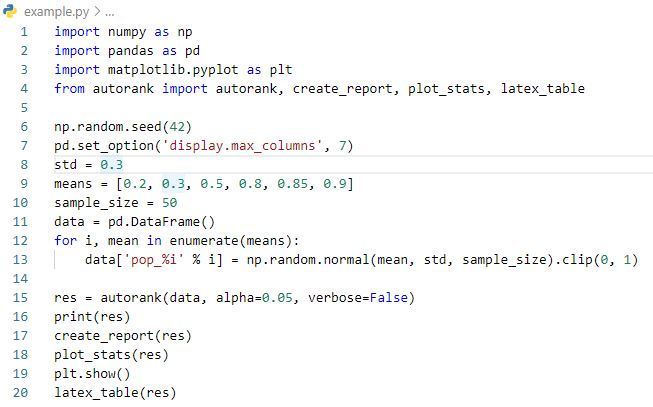
\includegraphics[width=10 cm]{autorank_example_code.png}
	\caption{example.py}
\end{figure}
\newpage
\section{Results}

Firstly, the result of autorank shows the content of the dataset.

\begin{figure}[!htbp]
	\centering
	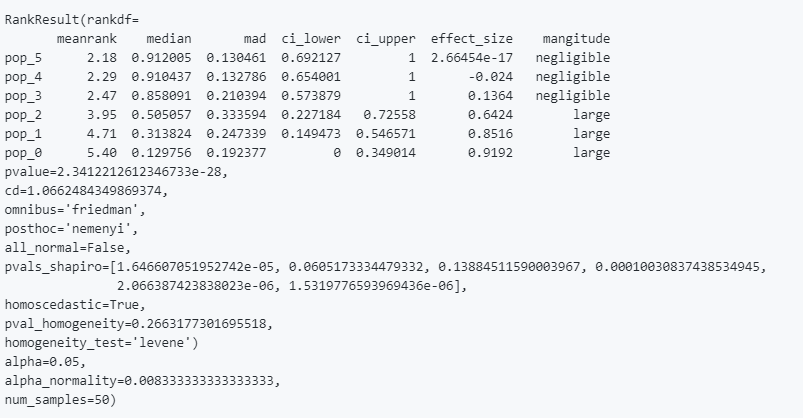
\includegraphics[width=11 cm]{contents.png}
	\caption{Contents of the dataset}
\end{figure}

Secondly, the statistical analysis of the dataset.
\begin{figure}[!htbp]
	\centering
	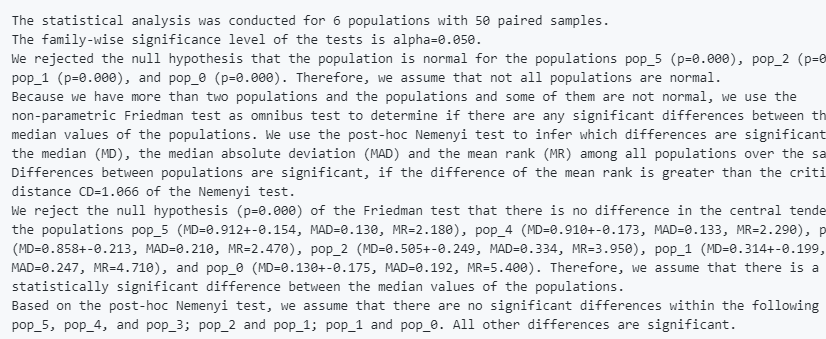
\includegraphics[width=11 cm, height=4 cm]{statistical_analysis1.png}
	\caption{Statistical Analysis}
\end{figure}

\newpage

Lastly, it displays the latex format of the dataset.
\begin{figure}[!htbp]
	\centering
	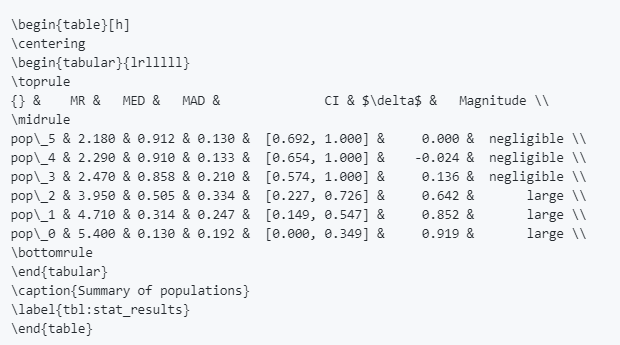
\includegraphics[width=15 cm]{latex.png}
	\caption{Latex format of the dataset}
\end{figure}

\section{Data Exploration}
\subsection{Dataset Summary}
This dataset has 17 columns and 11163 rows. Below is a detailed description of each column: 

\begin{itemize}

\item age: the age of group of ban customers
\item	job: type of job (admin., blue collar, entrepreneur, housemaid, management, retired, 'self-employed', 'services', 'student', 'technician', 'unemployed', 'unknown')
\item	marital: marital status (divorced, married, single, unknown; note: divorced means divorced or widowed)
\item	education: (primary, secondary, tertiary, and unknown)
\item	default: has credit in default? (no, yes, unknown)
\item	housing: has housing loan? (no, yes, unknown)
\item	loan: has personal loan? (no, yes, unknown)
\item	balance: Balance of the individual
\item	contact: contact communication type (cellular, telephone)
\item	month: last contact month of year 
\item	day: last contact day of the week 
\item	duration: last contact duration, in seconds (numeric). 
\item	campaign: number of contacts performed during this campaign and for this client 
\item pdays: number of days that passed by after the client was last contacted from a previous campaign 
\item	previous: number of contacts performed before this campaign and for this client 
\item outcome: outcome of the previous marketing campaign (failure, non-existent, success)
\item	deposit: has the client subscribed a term deposit? (yes or no)
\end{itemize}

\newpage
\subsection{Attributes Types}

\begin{table}[h!]
	\centering
	\begin{tabular}{|c|c|}
			\hline
		\textbf{Attributes}& \textbf{Types}\\
		\hline
			\hline
	age	&numeric\\
		\hline
	job	&categorical\\
		\hline
	marital&	categorical\\
		\hline
	education&	categorical\\
		\hline
	default	&categorical\\
		\hline
	housing	&categorical\\
		\hline
	loan	&categorical\\
		\hline
	contact	&categorical\\
		\hline
	balance	&numeric\\
		\hline
	contact	&unknown\\
		\hline
	month&	categorical\\
		\hline
	day	&numeric\\
	    \hline
	duration&	numeric\\
		\hline
	campaign&	numeric\\
		\hline
	pdays	&numeric\\
		\hline
	previous&	numeric\\
		\hline
	poutcome	&unknown\\
		\hline
	deposit&	categorical\\
		\hline
	\end{tabular}

	\caption{Attributes Types}
\end{table}

\newpage
\subsection{Implementing autorank in my dataset}
Banks use marketing campaigns as tools to focus on customer needs and their overall satisfaction strategically. However, different variables determine whether a marketing campaign will be successful or not. One of such avenue to develop a questionnaire during calls. Since duration of the call is the feature that most positively correlates with whether a potential client will open a term deposit or not. 

\begin{figure}[!htbp]
	\centering
	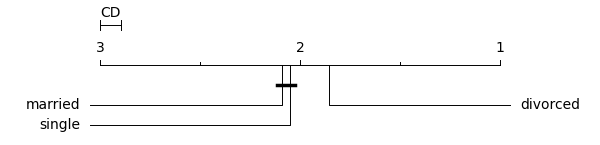
\includegraphics[width=15 cm]{stat_auto_rank.png}
	\caption{Autorank Plot}
\end{figure}

\newpage
The plot shows the number of contacts with different subset of customers during the campaign.
\begin{figure}[!htbp]
	\centering
	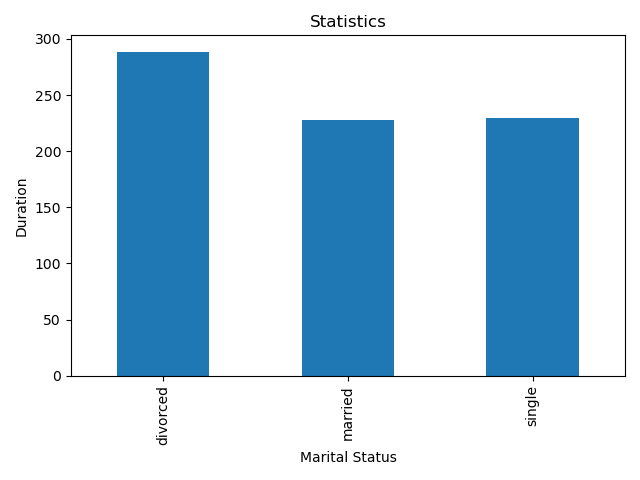
\includegraphics[width=15 cm]{mean.png}
	\caption{Bar Plot of the }
\end{figure}


\section{Conclusion}
The goal of Autorank is to simplify the statistical analysis for non-experts. Autorank takes care of all of the above with a single function call. Additional functions allow the generation of appropriate plots, result tables, and even of a complete latex document. All that is required is the data about the populations is in a Pandas dataframe.Overall, autorank statistical analysis involves evaluating and then summarizing the data into a mathematical form that was easy to implement in my dataset. 
\newpage

\begin{thebibliography}{999}

%reference 1
	\bibitem[Martinez, J. (2017)]{ref-software}
	Martinez, J. (2017). Bank Marketing Dataset. Retrieved July 31, 2020, from {\url{https://www.kaggle.com/janiobachmann/bank-marketing-dataset}}

   
%reference 2
	\bibitem[Herbold, S. (2020)]{ref-softwaree}
	S. Herbold (2020). Autorank: A Python package for automated ranking of classifiers. Journal of Open Source Software. https://doi.org/10.21105/joss.02173


\end{thebibliography}

\end{document}
